\documentclass[mathserif]{beamer}
\usepackage[utf8]{inputenc}
\usepackage{tikz}
\usetheme{Warsaw}
\usecolortheme{lily}

\title{Calendar Problem 15}
\author{Michael Peng}
\date{The Calendar Month, 2018}
\subtitle{The one with a parabola and an intersecting line}

\begin{document}
	\frame{\titlepage}
	
	\begin{frame}
		\frametitle{The Problem}
		
		A line $p$ with positive slope
		intersects the parabola $y=x^2$
		at $A(x_1, y_1)$ and $B(x_2, y_2)$, where $y_2 = y_1 + 16$. If $A$ and $B$ are $8\sqrt{5}$ units apart, what is the equation of the line $p$ in y-intercept form?
		
		\begin{figure}
			\centering
			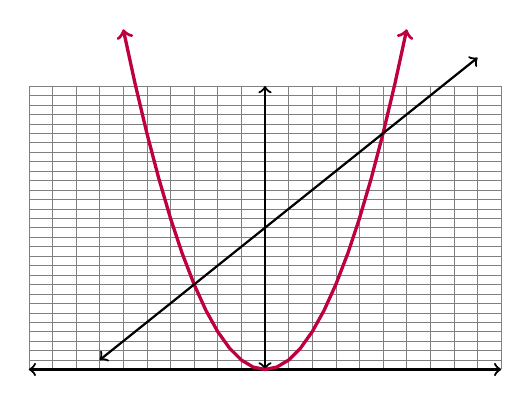
\begin{tikzpicture}[xscale=0.3,yscale=0.12]
			
			\draw[help lines] (-10,0) grid (10,30);
			\draw[<->][thick] (0,30) -- (0,0);
			\draw[<->][thick] (-10,0) -- (10,0);
			
			\draw[purple, very thick, <->, domain=-6:6] plot (\x, {\x*\x});
			\draw[black, thick, <->, domain=-7:9] plot (\x, {2*\x+15});
			\end{tikzpicture}
		\end{figure}
	\end{frame}

	\begin{frame}
		\frametitle{Deductions}
		
		\begin{center}
		\begin{tabular}{l | l}
			\centering
			$A(x_1,y_1)$ and $B(x_2,y_2)$ satisfy $y=x^2$ & Given intersection \\
			$y_2=y_1+16$ & Given \\
			$y_2-y_1=16$ & Subtraction Prop. of = \\
			$y_1=x_1^2$, $y_2=x_2^2$ & Substitution \\
			{\boldmath $x_2^2-x_1^2=16$} & Subtraction Prop. of = \\
			$\sqrt{(x_2-x_1)^2+(y_2-y_1)^2}=8\sqrt{5}$ & Distance Formula \\
			$(x_2-x_1)^2+(y_2-y_1)^2=(8\sqrt{5})^2=320$ & Multiplication Prop. of = \\
			$(x_2-x_1)^2+16^2=320$ & Substitution \\
			$(x_2-x_1)^2+256=320$ & Simplification \\
			$(x_2-x_1)^2=320-256=64$ & Subtraction Prop. of = \\
			{\boldmath $x_2-x_1=\sqrt{64}=\pm 8$} & Division Prop. of =
		\end{tabular}
	\end{center}
	
		$\therefore x_2^2-x_1^2=16, x_2-x_1=\pm 8$\\
		Split into Case A ($-8$) and Case B ($8$)
	
	\end{frame}

	\begin{frame}
		\frametitle{Case A}
		
		\textbf{Deduced:} $x_2^2-x_1^2=16, x_2-x_1=\pm 8, y_1=x_1^2, y_2=x_2^2$\newline
		\textbf{Current case:} $x_2-x_1=-8$
		
		\begin{center}
		\begin{tabular}{l | l}
			$x_2=-8+x_1=x_1-8$ & Addition Prop. of = \\
			$(x_1-8)^2-x_1^2=16$ & Substitution \\
			$x_1^2-16x_1+64-x_1^2=16$ & Factor \\
			$-16x_1+64=16$ & Simplify \\
			$-16x_1=16-64=-48$ & Subtraction Prop. of = \\
			$x_1=\frac{-48}{-16}=3$ & Division Prop. of = \\
			$x_2=3-8=-5$ & Substitution \\
			$y_1=3^2=9$ & Substitution \\
			$y_2=(-5)^2=25$ & Substitution
		\end{tabular}
	\end{center}
		$\therefore \text{Case A}: x_1=3,x_2=-5,y_1=9,y_2=25 \Rightarrow A(3,9), B(-5,25)$
\end{frame}

\begin{frame}
\frametitle{Case A: Contradiction}

\textbf{Deduced: } $A(3,9),B(-5,25)$\newline
\textbf{Given: } \textit{``A line $p$ with positive slope...''}

\begin{center}
	% TODO fix padding
	\begin{tabular}{l | l}
		Slope of $p$ is $\dfrac{y_2-y_1}{x_2-x_1}$ & Slope Formula \\
		Slope of $p$ is $\dfrac{25-9}{-5-3}$ & Substitution \\
		Slope of $p$ is $\dfrac{16}{-8}=-2$ & Simplification
		\end{tabular}
	
\end{center}

Slope of $p$ in Case A is negative, given positive. $\bot$!

\end{frame}
\begin{frame}
\frametitle{Case B}

	\textbf{Deduced:} $x_2^2-x_1^2=16, x_2-x_1=\pm 8, y_1=x_1^2, y_2=x_2^2$\newline
\textbf{Current case:} $x_2-x_1=8$

\begin{center}
	\begin{tabular}{l | l}
		$x_2=8+x_1$ & Addition Prop. of = \\
		$(8+x_1)^2-x_1^2=16$ & Substitution \\
		$64+16x_1+x_1^2-x_1^2=16$ & Factor \\
		$64+16x_1=16$ & Simplify \\
		$16x_1=16-64=-48$ & Subtraction Prop. of = \\
		$x_1=\frac{-48}{16}=-3$ & Division Prop. of = \\
		$x_2=8+(-3)=8-3=5$ & Substitution \\
		$y_1=(-3)^2=9$ & Substitution \\
		$y_2=5^2=25$ & Substitution
	\end{tabular}

\end{center}

$\therefore x_1=-3,x_2=5,y_1=9,y_2=25 \Rightarrow A(-3,9), B(5,25)$
\end{frame}

\begin{frame}
	\frametitle{Case B: Linear Equation}
	\framesubtitle{Only case possible}
	
	\textbf{Deduced:} $A(-3,9),B(5,25)$
	
	\begin{center}
		\begin{tabular}{l | l}
			Slope of $p$ is $\frac{y_2-y_1}{x_2-x_1}$ & Slope Formula \\
			Slope of $p$ is $\frac{y_2-y_1}{x_2-x_1}=\frac{25-9}{5-(-3)}$ & Substitution \\
			Slope of $p$ is $\frac{16}{8}=2$ & Simplification \\
		\end{tabular}
	\end{center}
	
	First point-slope, then slope-intercept for $p$: 
	
	\begin{center}
		\begin{tabular}{l | l}
			$y_2-y=m(x_2-x)$ & Point-slope formula \\
			$25-y=2(5-x)$ & Substitution \\
			$25-y=10-2x$ & Distributive Property \\
			$-y=10-2x-25=-15-2x$ & Subtraction Prop. of = \\
			$-1(-y)=-1(-15-2x)$ & Multiplication Prop. of = \\
			$y=15+2x=2x+15$ & Distributive Property
		\end{tabular}
	\end{center}

	$\therefore$ Equation for $p$ is $\boxed{y=2x+15}$
\end{frame}
\end{document}